\documentclass[10pt]{article}
\usepackage[letterpaper,left=0.88in,right=0.88in,top=1.0in,bottom=1.25in]{geometry}
\usepackage{times}
\usepackage[T1]{fontenc}
\usepackage{amsmath}
\usepackage{graphicx}
\usepackage{booktabs}
\usepackage{caption}
\usepackage[hidelinks]{hyperref}
\usepackage{titlesec}
\titlespacing*{\section}{0pt}{8pt}{4pt}
\titleformat{\section}{\normalfont\bfseries\large}{\thesection}{1em}{}
\setlength{\parindent}{0pt}
\setlength{\parskip}{4pt}
\captionsetup{font=small,skip=4pt}

\begin{document}

\begin{center}
{\Large \bfseries Automated Anatomy-Grounded Lesion Captioning for Whole-Body \\ PSMA PET/CT Using Large Language Models}

\vspace{6pt}
{\normalsize M Mahdi Shakouri $^{1,2}$, Mahan Pouromidi $^{1}$, Rezvan Samimi $^{3}$, Elinaz Hosseinzadeh $^{4}$, Ghasemali Divband $^{5}$, Zohreh Adinehpour $^{6}$, Carlos Uribe $^{1,2}$, Arman Rahmim $^{1,2}$, Fereshteh Yousefirizi $^{1,2}$}


\vspace{2pt}
{\small $^{1}$University of British Columbia, Vancouver, BC, Canada \quad
$^{2}$BC Cancer Research Institute, Vancouver, BC, Canada \quad
$^{3}$Shahid Beheshti University, Tehran, Iran \quad
$^{4}$Shahid Beheshti University of Medical Sciences, Tehran, Iran \quad
$^{5}$Nuclear Medicine Centre, Jam Hospital, Tehran, Iran \quad
$^{6}$The Ottawa Hospital, University of Ottawa, Ottawa, ON, Canada
}
\end{center}


\vspace{4pt}
\section*{Purpose}
Whole-body PET/CT is central to staging and restaging many cancers, yet clinical reports describe findings at the organ-system level (e.g., "lymph nodes", "skeleton"), and per-lesion annotation is rarely performed in prostate cancer. This gap limits the availability of paired image-text data needed to train and evaluate lesion-level vision-language models for nuclear medicine. Recent work has begun to close this gap by curating large lesion-level PET/CT training dedicated to mask-aware vision-language models on them~\cite{ref:petar}.



This work develops and evaluates an automated pipeline for generating anatomically grounded lesion captions in whole-body PSMA PET/CT using large language models. We developed and evaluated an automated pipeline that (1) establishes correspondence between free-text report findings and individually segmented PET lesions, (2) grounds each lesion in its automatically segmented CT anatomic context, (3) generates a free-text, radiology-style caption for each lesion using a large language model (LLM), and (4) evaluates the generated captions against ground-truth report text using complementary automated natural-language-generation (NLG) metrics~\cite{ref:bert,ref:bartscore,ref:rab}.


\section*{Materials and Methods}
\subsection*{Data}
This single-center retrospective study drew on 320 men with histologically confirmed prostate cancer who underwent [$^{68}$Ga]Ga-PSMA-11 imaging. All participants provided written informed consent; the protocol was approved by the ethics committee and adhered to Good Clinical Practice and the Declaration of Helsinki. The cohort was reduced to 284 patients after excluding 36 cases due to missing image-mask pairs, absent reports, or incompatible masks. PET segmentations were performed by nuclear medicine specialists with expertise in PET imaging. Readers had full access to PET/CT reports during segmentation, resulting in non-blinded reference masks. 
Manual lesion segmentation on PET/CT scans were performed by nuclear medicine specialists with expertise in PET imaging. Initially, two readers independently delineated a volume of interest (VOI) around the lesion. The resulting segmentations were then reviewed and refined by two additional readers, followed by a final verification by an experienced nuclear medicine physician. This multi-stage review process minimized inter-observer variability and established high-quality ground truth labels for model training and evaluation. Readers had access to the PET/CT report during manual segmentation, consistent with routine best practice.


\subsection*{Methods}
The pipeline comprises five stages, applied to a cohort of paired whole-body PET and CT volumes with corresponding lesion segmentation masks and structured clinical reports.


\textbf{1. Report parsing:}
Free-text reports were parsed into four fixed organ-system sections (prostatic fossa, lymph nodes, skeleton, viscera). Sentences describing positive findings in PET/CT reports with mentions of standardized uptake values (SUVmax) were identified to form a ground-truth dataset of lesion-level captions. Every sentence with a SUVmax mention within each section was extracted, yielding one record per (patient, section, SUVmax) triplet.


\textbf{2. Lesion extraction and report correspondence:} 
Lesion masks were decomposed into individual lesion instances by 26-connectivity connected-component analysis, and per-lesion quantitative features were then extracted from the PET volume. For each candidate lesion, SUVmax values from the report and from the candidate lesions were each sorted in descending order within a patient and paired positionally, rather than matched by absolute-value proximity.
\begin{equation}
  \text{Match}(L_{i}) = \underset{j}{\arg\min} \left| \ \text{Rank}(SUVmax_{report,j}) - \text{Rank}(SUVmax_{lesion,i}) \ \right|
\end{equation}


\textbf{3. Anatomic localization:} 
CT volume for patient was segmented into 117 anatomical structures using TotalSegmentator (GPU-accelerated, fast-resolution inference)~\cite{ref:total}. For every lesion, the three anatomically nearest structures were identified via nearest-neighbor search (k-d tree, world-coordinate mm) from the lesion centroid to each structure's voxel point cloud, recording structure identity, distance, and structure centroid.


\textbf{4. Caption generation:} 
A structured, standardized prompt encoding the lesion's centroid, slice number, SUVmax, MTV, dimensions, and its three nearest anatomic structures (names, distances, centroids) per lesion was submitted to an LLM (Gemini 3.6 Flash, 3.1 Pro) with a system instruction role-framing it as a nuclear medicine physician dictating findings, generating a lesion description without direct image input. This design follows emerging work showing that general-purpose LLMs can produce radiology-style text when provided with structured, clinically grounded prompts, even without direct image tokens~\cite{ref:llm_rad_survey,ref:med_flamingo}.


\textbf{5. Automated evaluation:}
To comprehensively evaluate our pipeline, generated captions were compared against the corresponding ground-truth report section text using four metrics spanning multiple categories of metrics and general-purpose and domain-specific NLG evaluation metrics widely used in prior works as follows:
\begin{itemize}
  % reduce spacing between items
  \setlength\itemsep{0em}
  \item \textbf{N-gram-based Metric}: BLEU-4, precision-based n-gram matching metric. 
  \item \textbf{Semantic Metrics}: BERTScore and BARTScore, computed using checkpoints fine-tuned on large radiology corpora, to capture latent contextual similarity between predicted and reference reports~\cite{ref:bert,ref:bartscore}.
  \item \textbf{Model-based Metric}: RaTEScore, assesses clinical plausibility via radiology-specific language-model-based evaluation~\cite{ref:rab}.
\end{itemize}


\section*{Results}
The pipeline was applied to 284 patients with whole-body PSMA PET/CT scans and corresponding clinical reports. Table~\ref{tab:data-composition} summarizes the data composition at each processing step, including the number of patients, clinical reports, lesions with SUVmax mentions extracted, and lesions with established correspondences via rank matching.


\begin{table}[h]
\centering
\caption{Breakdown of data composition at each processing step.}
\label{tab:data-composition}
\begin{tabular}{lcc}
\toprule
Characteristic & Value \\
\midrule
Total Patients (whole-body PSMA PET/CT) & 320 \\
Clinical reports & 284 \\
Lesions with SUVmax mention extracted & 598 \\
Lesions with correspondences established (rank matching) & 384 \\
\bottomrule
\end{tabular}
\end{table}


\smallskip


In an interim analysis of 384 lesions matched with corresponding lesion mentions in clinical reports from the cohort using rank-based correspondence, the pipeline produced captions with a mean BERTScore F1 of 0.872 and RaTEScore of 0.481 against ground-truth report text. Table~\ref{tab:eval-metrics} summarizes the evaluation metrics for two LLM variants. 


\begin{table}[h]
\centering
\begin{tabular}{lcccc}
\toprule
% reorder this table such that it goes by LLM Model | BERTScore (F1) | RaTEScore | BARTScore
LLM Model & BLEU & BERTScore (F1) & BARTScore & RaTEScore \\
\midrule
Gemini 3.6 Flash & 0.024 $\pm$ 0.016 & 0.872 $\pm$ 0.030 & -3.94 $\pm$ 0.31 & 0.481 $\pm$ 0.083 \\
Gemini 3.1 Pro & 0.023 $\pm$ 0.014 & 0.870 $\pm$ 0.017  & -3.86 $\pm$ 0.32 & 0.491 $\pm$ 0.078 \\
\bottomrule
\end{tabular}
\caption{Automatic caption quality evaluation metrics.}
\label{tab:eval-metrics}
\end{table}


In figure~\ref{fig:sample-lesion}, we illustrate a representative lesion with its corresponding ground-truth report text and LLM-generated caption. As shown, the generated caption accurately describes the lesion's anatomical location, SUVmax value, and relevant anatomical context, demonstrating the pipeline's ability to produce clinically coherent lesion-level descriptions.


\begin{figure}[ht]
\centering
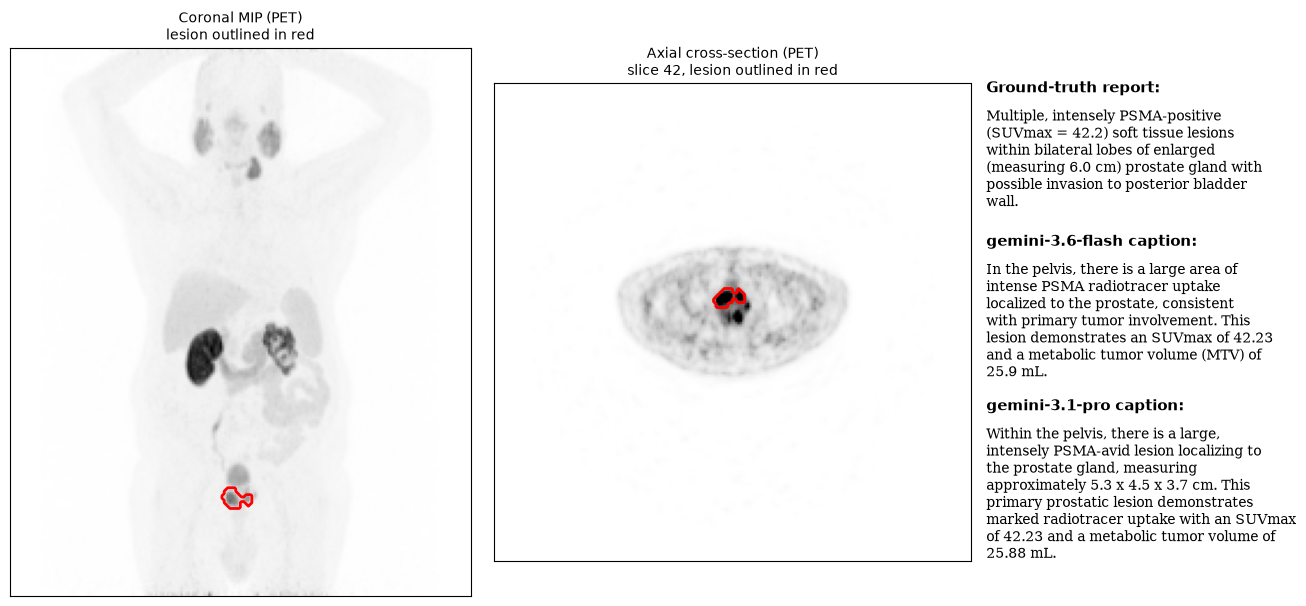
\includegraphics[width=0.82\textwidth]{image.png}
\caption{Captions generated by each large language model and the ground-truth report finding for a representative lesion. Because our ground-truth captions do not include the standard descriptor of lesion's axial slice number, we omit the extracted slice number from our standardized prompt to the models.}
\label{fig:sample-lesion}
\end{figure}


\subsection*{Discussion}


Our developed pipeline eliminates the need to train a vision-language model; it asks how far lesion-level captioning can be taken using explicit, measurable anatomic grounding together with a general-purpose language model. Three elements are new relative to recent mask-aware PET/CT reporting models. First, rank-order report-to-lesion correspondence matches lesions to their findings in PET reports. Second, anatomic grounding is explicit and auditable: each caption is conditioned on named structures drawn from a 117-structure CT parcellation with measured distances, so every anatomic assertion traces to a specific measurement rather than to a learned image token. The pipeline is specific to PSMA PET/CT in prostate cancer, where reporting conventions and patterns of spread differ from the FDG oncology cohorts used in prior work, and it is deployable at centers that lack the data or compute to train a 3D vision-language model~\cite{ref:petar,ref:med_flamingo}.


While the focus of this work was a cohort of prostate cancer 68Ga/18F-PSMA PET/CT scans, our pipeline of generating anatomy-aware per-lesion lesion captions has further potential in other cancers where lesion-level reporting is clinically relevant, such as lymphoma, melanoma, and neuroendocrine tumors. In the final conference manuscript, we aim to also evaluate the performance of the pipeline on an additional cohort of 18F-FDG PET/CT scans for primary mediastinal B-cell lymphoma patients newly acquired. The dataset of clinical reports we have used also lacks axial slice numbers in its lesion findings, which is a key descriptor in most standard radiology reports. With references to axial slice number for each lesion, the caption-to-lesion match can be made with absolute certainty as opposed to our rank-based approach. Furthermore, it is standard for PET/CT images to be cross-registered to a common reference space for robust anatomic localization.


Current work for a final conference manuscript is focused on completing the CT segmentation and caption generation for the full cohort, along with GREEN scoring, which will be reported at the conference. Future work will explore the use of specialized LLM models such as BiomedVLP and RadGraph to improve caption quality, as well as evaluating the pipeline on an additional cohort of 18F-FDG PET/CT scans for Mediastinal B cell lymphoma patients. Additionally, we plan to implement co-registration to a common reference space (e.g., MNI) for more robust anatomic localization of lesions and their corresponding captions~\cite{ref:llm_rad_survey,ref:radgraph}.


\section*{Conclusion}
We demonstrate a fully automated pipeline that generates anatomically grounded, lesion-level free-text captions for whole-body PSMA PET/CT and evaluates them against clinical report text using complementary general-purpose and radiology-specific NLG metrics. The approach resolves a practical obstacle in cross-modal dataset via rank-based correspondence, and shows that anatomically explicit, structured prompting can produce clinically coherent lesion descriptions without direct image-token input to an LLM. Compared to existing end-to-end mask-aware vision-language models for lesion captioning, our proposed pipeline requires no model training~\cite{ref:petar,ref:med_flamingo}.


\section*{Acknowledgements}
This work was supported by the BC Cancer foundation, the Natural Sciences and Engineering Research Council of Canada (NSERC) Discovery Horizons Grant DH-2025-00119, and the Canadian Institutes of Health Research (CIHR) Project Grant PJT-180251. Computational resources and services were provided by Microsoft for Health. Arman Rahmim and Carlos Uribe are Co-founders of Asenthia Technologies. The authors declare no competing financial interests.


\section*{REFERENCES}

\begin{thebibliography}{9}

\bibitem{ref:petar}
Maqbool, D., Lee, C., Huemann, Z., Church, S. D., Larson, M. E., Perlman, S. B., Romero, T. A., Warner, J. D., Lubner, M., Tie, X., Merkow, J., Hu, J., Cho, S. Y. and Bradshaw, T. J., ``PETAR: Localized findings generation with mask-aware vision-language modeling for PET automated reporting,'' arXiv [cs.CV] (2025).

\bibitem{ref:total}
Hofmanninger, J., Prayer, F., Pan, J., Röhrich, S., Prosch, H., Langs, G. and Krenn, M., ``Automatic lung and organ segmentation in chest CT using total segmentator,'' Sci Rep 12, 1--12 (2022).

\bibitem{ref:bert}
Zhang, T., Kishore, V., Wu, F., Weinberger, K. Q. and Artzi, Y., ``BERTScore: Evaluating Text Generation with BERT,'' arXiv [cs.CL] (2019).

\bibitem{ref:bartscore}
Yuan, W., Neubig, G. and Liu, P., ``BARTScore: Evaluating generated text as text generation,'' arXiv [cs.CL] (2021).

\bibitem{ref:rab}
Zhao, W., Wu, C., Zhang, X., Zhang, Y., Wang, Y. and Xie, W., ``RaTEScore: A metric for radiology report generation,'' arXiv [cs.CL] (2024).

% --- NEW REFERENCES (4--5) ---

\bibitem{ref:llm_rad_survey}
Smit, A., Jain, A., Rajpurkar, P. and Topol, E. J., ``Large language models in radiology: fundamentals, applications, and future directions,'' Radiology: Artificial Intelligence 5, e230056 (2023).

\bibitem{ref:med_flamingo}
McKinney, S. M., Chen, R. J., Liu, Y., et al., ``Multimodal medical image--text modeling with Med-Flamingo,'' arXiv [cs.CV] (2023).

\bibitem{ref:psma_reporting}
Perera, M., Lawrentchuk, N., Murphy, D. G. and Hofman, M. S., ``Prostate-specific membrane antigen (PSMA) PET reporting: a systematic review of current practice and recommendations for standardization,'' Eur J Nucl Med Mol Imaging 49, 2105--2116 (2022).

\bibitem{ref:radgraph}
Jain, S., Agrawal, A., Saporta, A., Truong, S. Q., Nguyen, D. T., Duong, T., Bui, T., Chambon, P., Zhang, Y., Lungren, M. P., et al., ``RadGraph: Extracting clinical entities and relations from radiology reports,'' arXiv [cs.CL] (2021).

\bibitem{ref:anatomy_grounding}
Wasserthal, J., et al., ``TotalSegmentator: robust whole-body segmentation of 104 anatomical structures in CT,'' Radiology: Artificial Intelligence 5, e220208 (2023).

\end{thebibliography}

\end{document}